% Worktree isolation — before/after. Left (rose): two agents on a shared tree
% collide on one file. Right (green): each agent gets its own worktree, no overlap.
% Warm-Tol palette; before=rose / after=green framing.
\documentclass[tikz,border=4mm]{standalone}
\usepackage{tikz}
\usetikzlibrary{positioning, arrows.meta, calc}

\definecolor{warmblue}{HTML}{3B6FA0}
\definecolor{warmrose}{HTML}{C06858}
\definecolor{warmgreen}{HTML}{4A7E3F}

\begin{document}
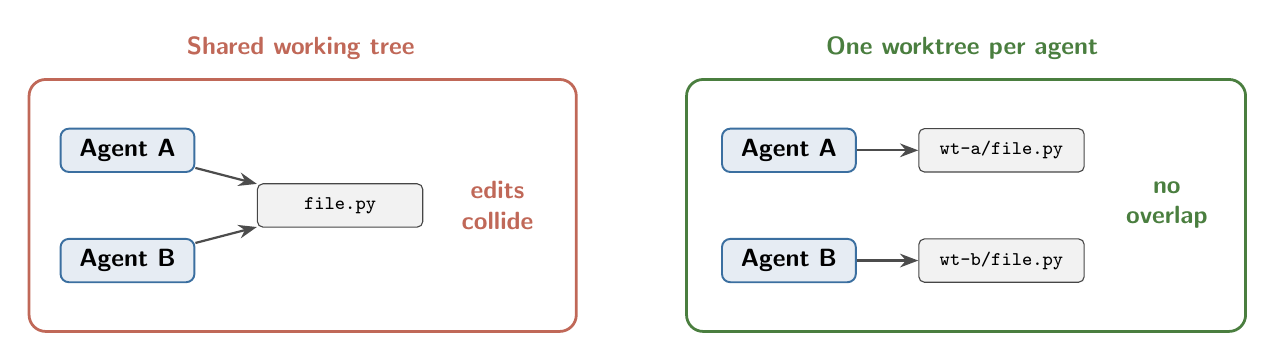
\begin{tikzpicture}[
  font=\sffamily,
  agent/.style={draw=warmblue, fill=warmblue!13, rounded corners=3pt,
    minimum width=1.7cm, minimum height=0.55cm, font=\sffamily\small\bfseries, line width=0.7pt},
  file/.style={draw=gray!55!black, fill=gray!10, rounded corners=2pt,
    minimum width=2.1cm, minimum height=0.55cm, font=\sffamily\scriptsize\ttfamily},
  arrow/.style={-Stealth, thick, draw=gray!60!black},
  ptitle/.style={font=\sffamily\small\bfseries},
]

% ---- LEFT: shared tree (collision) ----
\node[agent] (la) at (0,0.7) {Agent A};
\node[agent] (lb) at (0,-0.7) {Agent B};
\node[file] (lf) at (2.7,0) {file.py};
\draw[arrow] (la) -- (lf);
\draw[arrow] (lb) -- (lf);
\node[ptitle, text=warmrose, align=center] (lv) at (4.7,0) {edits\\collide};
\draw[rounded corners=6pt, draw=warmrose, line width=1pt] (-1.25,-1.6) rectangle (5.7,1.6);
\node[ptitle, text=warmrose] at (2.2,2.0) {Shared working tree};

% ---- RIGHT: worktrees (isolated) ----
\node[agent] (ra) at (8.4,0.7) {Agent A};
\node[agent] (rb) at (8.4,-0.7) {Agent B};
\node[file] (rfa) at (11.1,0.7) {wt-a/file.py};
\node[file] (rfb) at (11.1,-0.7) {wt-b/file.py};
\draw[arrow] (ra) -- (rfa);
\draw[arrow] (rb) -- (rfb);
\node[ptitle, text=warmgreen, align=center] (rv) at (13.2,0) {no\\overlap};
\draw[rounded corners=6pt, draw=warmgreen, line width=1pt] (7.1,-1.6) rectangle (14.2,1.6);
\node[ptitle, text=warmgreen] at (10.6,2.0) {One worktree per agent};

\end{tikzpicture}
\end{document}
